\documentclass[12pt, letterpaper]{article}
\usepackage[spanish]{babel}
\usepackage[utf8]{inputenc}
\usepackage{graphicx}
\usepackage{amssymb}
\graphicspath{{./imagenes/}}
\usepackage{xcolor}

%Paquetes para símbolos y entornos matematicos. En este documento se usa para poder usar el tag \begin{align} y \begin{align*} que permiten alinear expresiones matemáticas
\usepackage{amsmath}
\usepackage{amssymb}
%paquete que permite el uso de del argumento H al momento de insertar imágenes
\usepackage{float}

%comando para especificar el título del documento 
\title{Matemáticas para las Ciencias Aplicadas I}

%comando para especificar el autor del documento
\author{Pérez Romero Natalia Abigail}

%comando para especificar la fecha del documento
\date{\today}
%--------------Fin preámbulo--------------

%------------Inicio documento-------------
\begin{document}
%comando que genera el titulo con los datos especificados en el preámbulo
\maketitle
\textbf{Tarea X. Ejercicios del libro Cálculo. Una variable de Thomas J.R, George B.}

\textbf{Ejercicios 7, 9, 16 y 57 de  la sección 2.3 La definición formal de Límite}

\textbf{7.} Use la gráfica para encontrar un $\delta > 0$ tal que para toda $x$\\
$0 < | x - x_0| < \delta \rightarrow | f(x)-L |<\epsilon$\\

Si $x_0 = 5$ y en la gráfica se observa que $x_0 - \delta = 4.9$ y $x_0 + \delta = 5.1$, lo que nos indica que se puede tomar cualquier $\delta$ en el intervalo $(4.9, 5.1)$ y séra valido, por ejemplo $\delta = 4.91$

\begin{figure}[tbh]
\centering
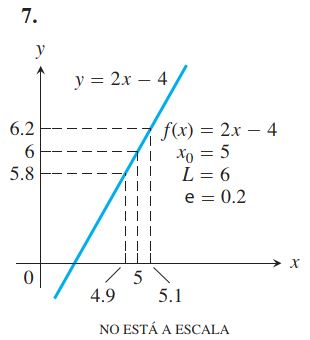
\includegraphics[width=15em]{t10uno}
\end{figure}

\newpage
\textbf{9.} Use la gráfica para encontrar un $\delta > 0$ tal que para toda $x$\\
 $0 < | x - x_0| < \delta \rightarrow | f(x)-L |<\epsilon$\\

Si $x_0 = 1$ y en la gráfica se observa que $x_0 - \delta = \frac{9}{16}$ y $x_0 + \delta = \frac{25}{16}$,  lo que nos indica que se puede tomar cualquier $\delta$ en el intervalo $(\frac{9}{16}, \frac{25}{16})$ y séra valido, por ejemplo $\delta = \frac{10}{16}$

\begin{figure}[tbh]
\centering
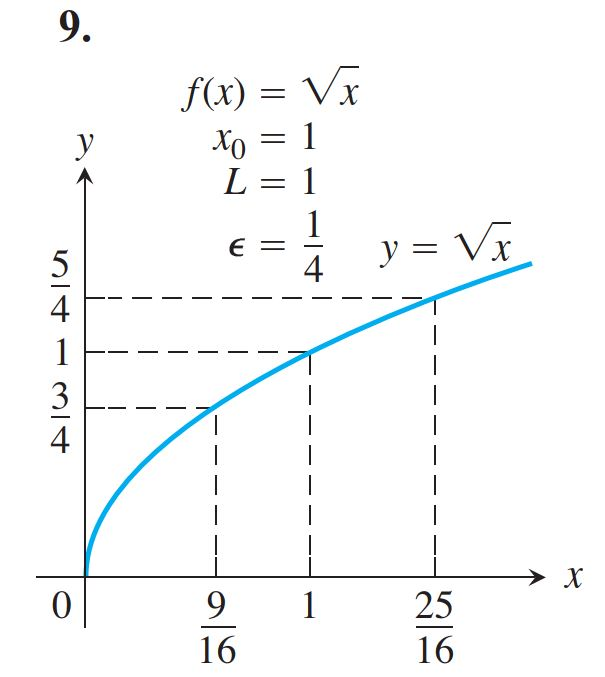
\includegraphics[width=15em]{t10dos}
\end{figure}

\textbf{16. Determinación algebraica de deltas}. Encuentre, en cada caso, un intervalo abierto alrededor de $x_0$ en donde se cumpla la desigualdad  $|f(x) - L| < \epsilon$. Después dé un valor para $\delta > 0$ tal que para toda $x$ que satisfaga $0 < |x - x_0| < \delta$ se cumpla la desigualdad $|f(x) - L| < \epsilon $

\begin{align*}
	f(x) = 2x - 2, L = -6, x_0 = -2, \epsilon = 0.02
\end{align*}

\begin{align*}
	0 < | x - x_0| < \delta \rightarrow | f(x)-L |<\epsilon\\
	\text{Resolver desigualdad}| f(x)-L |<\epsilon\\
	| (2x - 2) - (-6) |< (0.02)\\
	| 2x + 4 |< 0.02\\
	-0.02 < 2x + 4 < 0.02\\
	-0.02 - 4 < 2x < 0.02 - 4\\
	-0.02 - 4 < 2x < 0.02 - 4\\
	-4.02/ 2 < x < -3.98/ 2\\
	- 2.01 < x < - 1.99
\end{align*}

La desigualdad se satisface para toda $x$ en el intervalo abierto (-2.01,-1.99) , de manera que también se satisface para toda $x \neq -2$ en este intervalo.
Encontrar un valor de $\delta > 0 $ para colocar el intervalo cerrado $-2 - \delta < x < -2 + \delta$ (con centro en $x_0 = -2$) dentro del intervalo $(-2.01,-1.99)$. Si tomamos $\delta = -2.012$ o cualquier número en el intervalo,  la desigualdad $0 < | x + 2| < \delta$ colocará automáticamente a $x$ entre -2.01 y -1.99 para hacer que  $| 2x + 4 |< 0.02$ 

\begin{align*}
	0 < | x + 2| < - 2.012 \rightarrow | 2x + 4 |< 0.02
\end{align*}

\textbf{57. Sea}
$$f(x) = \left\{
\begin{array}{c l}
 x,  & x < 1\\
 x+1  & x >1
\end{array}
\right.
$$

\begin{figure}[tbh]
\centering
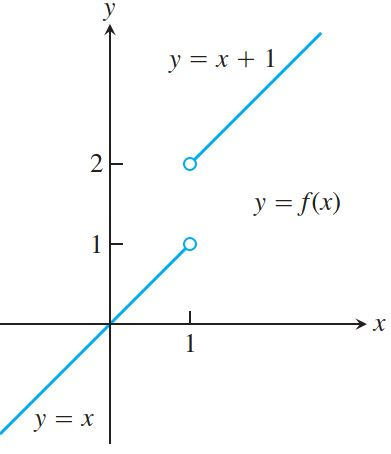
\includegraphics[width=15em]{t10tres}
\end{figure}

\textbf{a.} Sea $\epsilon = 1/2$. Demuestre que ninguna posible $\delta > 0$ satisface la condición siguiente:\\
Para toda $x$, $0 < | x - 1| < \delta \rightarrow | f(x) - 2 |< 1/2.$\\

Resuelvo la desigualdad para encontrar un intervalo abierto que contenga a $x_0 = 1$ en el que la desigualdad se satisfaga para toda $x \neq x_0$
\begin{align*}
	| f(x) - 2 |< 1/2 \\
	| x + 1 - 2 |< 1/2\\
	| x - 1 |< 1/2\\
	-1/2< x - 1< 1/2\\
	-1/2+ 2/2 < x < 1/2+2/2\\
	1/2 < x < 3/2
\end{align*}

La desigualdad 	$| f(x) - 2 |< 1/2$ se satisface para toda $x\neq 1$ en el intervalo (1/2 , 3/2)

Esto es, para cada $\delta > 0$, compruebe que hay un valor de $x$ tal que \\
 $0 < | x - 1| < \delta$ y $| f(x) - 2 |\geq 1/2$\\

Resuelvo la desigualdad para encontrar un intervalo abierto que contenga a $x_0 = 1$ en el que la desigualdad se satisfaga para toda $x \neq x_0$
\begin{align*}
	| f(x) - 2 | \geq 1/2 \\
	| x - 1 | \geq 1/2 \\
	 (x - 1) \geq 1/2 \text{ o }  (x-1)\leq -1/2\\
		x  \geq (1/2+2/2) \text{ o }  x-\leq (-1/2+ 2/2)\\
		x  \geq 3/2 \text{ o }  x \leq 1/2\\
\end{align*}

Es decir que la desigualdad |$ f(x) - 2 | \geq 1/2$ se satisface para toda $x\neq 1$ en el intervalo $(-\infty, 1/2] \cup [3/2, \infty)  $

Si tomará una $0< \delta > 1/2$, tal que $f(x_0+1/2)$ estará en el intervalo $[3/2, \infty)$

Si tomará una $0 < \delta < 1/2$, tal que $f(x_0 - 1/2)$ estará en el intervalo $(-\infty, 1/2]$


Esto probará que $\lim_{x \to 1} f(x) \neq 2$

\textbf{b.} Demuestre que $\lim_{x \to 1} f(x) \neq 1$

Supongo que $\lim_{x \to 1} f(x) = 1$, entonces $0 < | x - 1| < \delta \rightarrow | x - 1 | <\epsilon$\\

Y dada un $\epsilon = 1/2$
Resuelvo la desigualdad para encontrar un intervalo abierto que contenga a $x_0 = 1$ en el que la desigualdad se satisfaga para toda $x \neq x_0$
\begin{align*}
	| f(x) - 1 |< 1/2 \\
	| x - 1 |< 1/2\\
	- 1/2 <  x - 1 < 1/2\\
	- 1/2 + 2/2 <  x  < 1/2 + 2/2\\
	 1/2 <  x  < 3/2\\
\end{align*}
La desigualdad 	$| f(x) - 1 |< 1/2$ se satisface para toda $x\neq 1$ en el intervalo (1/2 , 3/2)\\

$| f(x) - 2 | > 1/2$\\
Resuelvo la desigualdad para encontrar un intervalo abierto que contenga a $x_0 = 1$ en el que la desigualdad se satisfaga para toda $x \neq x_0$
\begin{align*}
	| f(x) - 1 | > 1/2 \\
	| x - 1 | > 1/2\\
	- 1/2 >  x - 1 > 1/2\\
	- 1/2 + 2/2  >  x  > 1/2 + 2/2\\
	 1/2  >  x  > 3/2\\
\end{align*}
La desigualdad 	$| f(x) - 1 | > 1/2$ se satisface para toda $x\neq 1$ en el intervalo $(-\infty, 1/2) \cup (3/2, \infty)$\\

Si tomará una $0< \delta > 1/2$, tal que $f(x_0+1/2)$ estará en el intervalo $[3/2, \infty)$
Si tomará una $0 < \delta < 1/2$, tal que $f(x_0 - 1/2)$ estará en el intervalo $(-\infty, 1/2]$
Esto probará que $\lim_{x \to 1} f(x) \neq 1$

\textbf{c.} Compruebe que $\lim_{x \to 1} f(x) \neq 1.5$

Supongo que $\lim_{x \to 1} f(x) = 1$, entonces $0 < | x - 1| < \delta \rightarrow | x - 1 | <\epsilon$\\
Y dada un $\epsilon = 1/2$

Resuelvo la desigualdad para encontrar un intervalo abierto que contenga a $x_0 = 1$ en el que la desigualdad se satisfaga para toda $x \neq x_0$
\begin{align*}
	| f(x) - 3/2 | < 1/2 \\
	| x - 3/2 |< 1/2\\
	- 1/2 <  x - 3/2 < 1/2\\
	- 1/2 + 3/2 <  x  < 1/2 + 3/2\\
	   1 <  x  < 2\\
\end{align*}
La desigualdad $| f(x) - 3/2 |< 1/2$ se satisface para toda $x\neq 1$ en el intervalo (1 , 2)\\

$| f(x) - 3/2 | > 1/2$\\
Resuelvo la desigualdad para encontrar un intervalo abierto que contenga a $x_0 = 1$ en el que la desigualdad se satisfaga para toda $x \neq x_0$
\begin{align*}
	| f(x) - 3/2 | > 1/2 \\
	| x - 3/2 | > 1/2\\
	- 1/2 >  x - 3/2 > 1/2\\
	- 1/2 + 3/2  >  x  > 1/2 + 3/2\\
	 1  >  x  > 2\\
\end{align*}
La desigualdad 	$| f(x) - 3/2 | <1/2$ se satisface para toda $x\neq 1$ en el intervalo $(-\infty, 1) \cup (2, \infty)$\\

Si tomará una $0< \delta > 1/2$, tal que $f(x_0+1/2)$ estará en el intervalo $[2, \infty)$
Si tomará una $0 < \delta < 1/2$, tal que $f(x_0 - 1/2)$ estará en el intervalo $(-\infty, 1]$
Esto probará que $\lim_{x \to 1} f(x) \neq 1.5$
\end{document} 